\documentclass{scrreprt}

\usepackage[italian]{babel}
\usepackage[utf8]{inputenc}
\usepackage{parskip}
\usepackage{graphicx}

%\title{Report del Progetto di Compilatori e Interpreti}
%\date{}
%\author{Giuseppe De Palma  \and Andrew Memma  \\ \\Corso di Laurea Magistrale in Informatica}
%0000854846
%1900068459

\begin{document}

\begin{titlepage}
	\centering
	{\scshape\LARGE Alma Mater Studiorum\\Università di Bologna \par}
	\vspace{1cm}
	{\scshape\Large Report\par}
	\vspace{1.5cm}
    {\huge\bfseries Progetto di Compilatori e Interpreti\par}
    \vspace{0.5cm}
    {\scshape\Large Corso di Laurea Magistrale in Informatica\par}
	\vspace{2cm}
    {\Large\itshape Giuseppe De Palma\par}
    {\Large 0000854846\par}
	\vspace{0.5cm}    
    {\Large\itshape Andrew Memma\par}
    {\Large1900068459\par}
    \vfill
    
    % Bottom of the page
	{\large \today\par}
\end{titlepage}

\tableofcontents

\chapter{Introduzione}
Il lavoro presentato riguarda un compilatore per un semplice linguaggio di programmazione ad oggetti: FOOL. Il progetto è parte dell'esame del corso ``Compilatori e Intepreti'' della Magistrale in Informatica, Università di Bologna. Il lavoro è stato svolto da 2 studenti del suddetto corso.

L'obiettivo di tale progetto è volto allo studio dello sviluppo e funzionamento dei compilatori. Partendo dal testo di un programma scritto in FOOL, il compilatore lo analizza sia per ricavarne le informazioni necessarie per generare codice eseguibile, sia per controllarne la correttezza. 
Si fa uso di diverse tecniche per cercare errori nei programmi (a tempo di compilazione). In particolare, il linguaggio si avvale di un semplice sistema di tipi e il compilatore esegue un controllo di tipi statico che permette di segnalare all'utente errori di tipo. Con questo controllo si ha il vantaggio di evitare
i cosiddetti errori \textit{untrapped} e una parte degli errori \textit{trapped}, cioè l'insieme degli errori ``proibiti''.\footnote{Distinguiamo due generi di errore in un programma: errori \textit{trapped}, ovvero quelli che provocano il fallimento della computazione, e gli errori	\textit{untrapped}, che non	presentano sintomi immediatamente visibili, e sono perciò più insidiosi. 
Al primo tipo appartengono, ad esempio, la divisione per zero o un accesso proibito alla memoria; al secondo la lettura erronea di una porzione non significativa della memoria.}

FOOL non è l'unico linguaggio utilizzato, infatti il compilatore deve generare del codice eseguibile (da un elaboratore) partendo da un programma scritto in FOOL. Questo nuovo codice è scritto in un linguaggio \textit{assembly} per una \textit{stack virtual machine} con registri (SVM), il quale offre istruzioni per alcuni calcoli aritmentici, per gestione di \textit{stack} e \textit{heap} e salti condizionati. In accordo con le estensioni fatte a FOOL, anche il linguaggio SVM è stato arricchito.

\section{Outline}
Nei capitoli successivi è presentato in modo approfondito il progetto e le sue caratteristiche principali. Nel capitolo successivo viene descritta la struttura del compilatore e come utilizzarlo e una breve analisi sulle diverse parti che lo costituiscono. 
Il capitolo 3 discute la grammatica del linguaggio e come da questa si ricavano le informazioni per proseguire con la compilazione. Nel capitolo 4 è discussa l'analisi semantica, in particolare \textit{scope} e \textit{type checking}. Infine, nel capitolo 5, la generazione del codice assembly e la sua esecuzione.

\chapter{Descrizione del Progetto}
\section{Struttura}
Il compilatore è stato sviluppato nel linguaggio di programmazione Java, utilizzando il \textit{tool} Antlr nella sua versione 4.6 per la generazione automatica di \textit{lexer} e \textit{parser}.
Avendo, quindi, definito la grammatica di FOOL (nel file \textit{FOOL.g4}), il \textit{tool} genera le varie classi che permettono di effettuare l'analisi lessicale e sintattica sui programmi scritti in FOOL.
In questo modo la creazione di \textit{tokens} e la creazione dell'albero astratto di sintassi (\textit{Abstract Syntax Tree}) sono già gestite da Antlr, il quale fornisce due metodi per visitare ed utilizzare l'albero: i \textit{visitor} e \textit{listener} design patterns.
Per questo progetto il \textit{visitor pattern} è stato scelto per visitare l'albero ed ottenere il necessario per effettuare l'analisi semantica e la generazione di codice.

Il progetto è stato strutturato in diversi package, partendo dal codice fornito dal professore:
\begin{itemize}
    \item ast: contiene le classi che rappresentano i nodi dell'albero visitato con il Visitor di \textit{Antlr}. 
            L'interfaccia Node rappresenta il concetto di nodo dell'albero astratto sintattico, in particolare dichiara tre metodi:
            \textit{checkSemantics}, \textit{typeCheck}, \textit{codeGeneration}. Le classi usate per i vari tipi di nodo implementano questa interfaccia.
    \item codeexecution: si occupa della esecuzione del codice e della gestione della memoria. In particolare la classe VirtualMachine interpreta il codice (SVM) generato dalle istruzioni in FOOL.
    \item lib: contiene la libreria \textit{Antlr 4.6}, necessaria per l'esecuzione del compilatore.
    \item parser: contiene \textit{FOOL.g4} e le diverse classi create da \textit{Antlr}.
    \item svm:  contiene \textit{SVM.g4} e le diverse classi create da \textit{Antlr}.
    \item type: contiene le classi che rappresentano i tipi dei costrutti FOOL: IntType, BoolType, ClassType, VoidType.
    \item util: contiene in particolare la classe \textit{Enviroment} che offre varie strutture dati di utilità e la \textit{Symbol Table}, e la classe FOOLlib che oltre ad alcuni metodi utili
            per la generazione del codice, offre il metodo \textit{isSubType} per il controllo dei tipi delle espressioni FOOL.
\end{itemize}

Il file ``CompilerLauncher.java'' è il punto d'entrata del compilatore.

\section{Istruzioni Per l'Utilizzo}
\begin{enumerate}
    \item Importare il progetto in \textit{Eclipse} oppure \textit{IntelliJ}.
    \item Se il progetto presenta problemi, aggiungere nel \textit{Build Path} la libreria \textit{Antlr} contenuta nella cartella \textit{lib}.
        Da Eclipse, tasto destro sulla cartella del progetto, \textit{Configure Build Path} e da lì aggiungere la libreria.
    \item Il file ``prova.fool'' nella cartella \textit{Tests} contiene il codice FOOL che il compilatore utilizza. Scrivere lì il proprio codice. 
        Il compilatore legge il file ``prova.fool'' e, in seguito ai controlli di errori, crea il file ``prova.fool.asm'' con il codice SVM corrispondente.
    \item In caso di errori in un qualunque punto del processo (errori lessicali, sintattici, di scope, di tipi), l'esecuzione verrà interrotta e verrà mostrato l'errore
        nel terminale.
    \item Se nel codice FOOL vengono utilizzati comandi \textit{print}, viene mostrata l'espressione da stampare nel terminale. 
\end{enumerate}

\chapter{Sintassi}

\section{Definizione della Sintassi}
Le regole sintattiche che definiscono ciò che costituisce un programma scritto ``correttamente'' si 
trovano nel file di grammatica di \textit{FOOL.g4} nel package parser.

La serie di regole grammaticali di cui \textit{FOOL.g4} è composto fungono da sostituzioni. Essi associano simboli
non-terminali sia aa terminali (stringhe letterali), sia ad altri non-terminali, che a loro volta vengono associati 
ad altre sostituzioni, per rendere possibile, infine, l’associazione di un programma in FOOL a una combinazione legale
di regole grammaticali che definiscono il linguaggio. 
È questo il compito del \textit{lexer} e del \textit{parser}, che vengono discussi successivamente, cioè della 
rappresentazione di una serie di stringhe letterali in regole grammaticali opportune. 

\section{Caratteristiche Grammaticali}

La potenza espressiva della grammatica è fornita in gran parte dalla notazione sintattica accettata da 
\textit{ANTLR}. Essa supporta quella usata nella scrittura di espressioni regolari, le regex, che utilizza i 
simboli per quantificare le istanze di un’espressione indicata, quali `` ? '', `` * '', `` + '' e `` $\mid$ ''. 

Questa espressività si è vista anche nell'abilità di allocare regole di precedenza alle espressioni 
grammatiche desiderate. Il caso esemplare in FOOL è la precedenza data alle operazioni di divisone e 
moltiplicazione sopra quelle di addizione e sottrazione tramite la distinzione tra i ``factor'' e i ``term''. 
\\

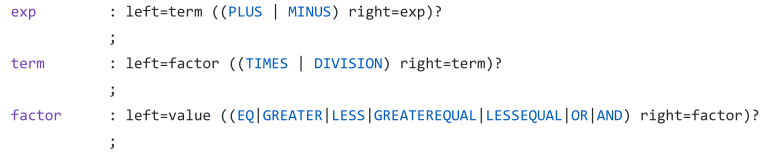
\includegraphics[width=\linewidth]{fool_exp_term_factor.png}
 
Inoltre, durante il corso dello sviluppo di questo progetto
FOOL è stato reso ancor più espressivo con l'aggiunta di classi, di statements e della possibilità di utilizzare espressioni multiple nel corpo di funzioni 
e dei let in (anche mischiando statements ed exps). 

Nella progettazione di queste capacità aggiuntive, decisioni riguardo le loro convenzioni sintattiche 
legali sono state prese tenendo conto di un bilancio tra espressività e l'attuabilità 
dell'implementazione. Un esempio di questo è il cambiamento alla sintassi delle dichiarazioni di 
funzioni, che adesso richiede i propri incapsulamento tra parentesi graffe.
Questo è stato giudicato necessario per eliminare ogni ambiguità nei limiti delle funzioni. 

Similarmente, la dichiarazione dei campi e delle funzioni nelle classi vanno scritti tra parentesi e 
parentesi graffe, rispettivamente. Se non vi sono dichiarati nessun campo o funzione, le parentesi tra 
cui sarebbero stati scritti non vanno scritte. Così rimuove il bisogno di scrivere parentesi vuote, 
influenzando la leggibilità. 

Un aspetto importanto sviluppato nella grammatica di FOOL è l'introduzione delle statement, 
ovvero assegnamenti a variabili già esistenti, e l'abilità di utilizzarle liberamente con le 
espressioni sia nelle funzioni che nel corpo del programma. L'aggiunta di tale capacità era 
considerata del tutto essenziale al linguaggio FOOL, permettendo come minimo un funzionamento
 di base di manipolazione di variabili. 

Permettere un utilizzo libero di diversi tipi di istruzioni, di fatto, causava delle difficoltà nella sua implementazione. Un 
esempio è l'ambiguità che creava nella localizzazione del valore di ritorno di una funzione, essendo 
quello ritornato dalla sua ultima riga di codice. Dato il modo in cui \textit{Antlr} facilita l'’accesso alle righe 
del codice FOOL, raggruppandole secondo le loro categorie (in questo caso ``espressioni'' o 
``statements'') per determinare se l’ultima istruzione fosse un'espressione oppure una statement era facile nel caso una funzione potesse avere soltanto o espressioni oppure statements. Potento usare
in modo libero un qualsiasi numero di espressioni e statements, invece, ha richiesto un approccio diverso, specialmente per determinare
 il valore di ritorno. Considerando i due tipi di comandi come un unica sequenza di istruzioni (Node) ha permesso di poter trascurare le due categorie
 e piuttosto controllare il tipo dell'ultima istruzione nella sequenza.

\section{Controllo della Sintassi}

Il codice fornito in input deve aderire alla sintassi definita. L’obiettivo di \textit{Antlr} è quello di controllare che il programma sia 
corretto sintatticamente, in modo tale da avere un programma adeguato per la 
verifica semantica successiva. Per raggiungere tale scopo, si rappresenta il programma 
fornito come un albero AST (\textit{abstract syntax tree}), il quale fungerà da rappresentazione strutturata 
del programma per facilitare la sua analisi. 

Il primo passo in questo processo è la conversione del programma da formato testo in un stream dei 
\textit{tokens}, compiuto dal \textit{lexer}. Il flusso consiste di valori che corrispondono a termini categorizzati del 
linguaggio FOOL quali identificatori, interi o caratteri grammaticali. Questa rappresentazione del 
programma permette più facilmente al \textit{parser} di compiere il suo compito, ovvero quello di applicare 
le regole grammaticali definite nel file \textit{.g4} al flusso. Trasformando i \textit{token} del flusso, cioè i terminali 
della grammatica FOOL, in non-terminali che sono associati a tali \textit{token}, vengono annotati creando 
una struttura dati di contesti grammaticali. Ciascuno di questi è un nodo nella struttura. 

La radice di questo albero di contesti viene passato al \textit{FOOLNodeVisitor} che visita ognuno dei suoi 
contenuti. Accompagnato ad ogni visita è la generazione di uno o più nodi del AST, che infine 
costituiranno l’AST finale, pronto per l’analisi semantica.

Da notare che questo processo fallisce in caso di input sintatticamente errato. Programmi 
che non aderiscono alla grammatica definita causeranno eccezioni della fase
del parser, che fallirà ad associare con successo le regole ai suoi token. 

\chapter{Semantica}
L'analisi semantica si occupa del controllo dello scope e del controllo dei tipi, che vengono eseguiti mediante i metodi \textit{checkSemantics} e \textit{typeCheck}, 
ereditati dall'interfaccia Node da tutte le classi che rappresentano i nodi dell'AST.

\section{Scope}
Questo primo controllo, tramite \textit{checkSemantics}, serve per accertarsi del corretto utilizzo di variabili, funzioni e classi. Ad esempio, se una variabile viene utilizzata
ma non è mai stata dichiarata, l'errore viene incontrato in questa fase dell'esecuzione del compilatore. 

Dopo aver visitato l'albero di sintassi e instanziati i nodi appropriati, 
viene invocato \textit{checkSemantics} dal punto di entrata dell'albero (la radice), che sarà un nodo ``\textit{Prog}'' (ProgExpNode, ProgLetInNode o ProgClassNode). 
Esso invocherà lo stesso metodo sul nodo figlio, il quale continuerà ad invocare sul proprio figlio e così via, fino alle foglie dell'albero.

In particolare, i controlli vengono fatti mediante una \textit{Symbol Table}, cioè una lista di hash tables nella classe Environment. Una hash table rappresenta uno scope nel programma,
nel quale vengono inseriti gli identificatori di variabili, funzioni e classi associati alle proprie \textit{STEntry}. I vari scope sono indicizzati tramite l'intero \textit{nesting level}, che parte da 0 quando 
la Symbol Table è vuota ed incrementa di 1 ad ogni inserimento di hash table (quando si entra in nuovo scope). Gli oggetti STEntry contengono il nesting level, il tipo e l'\textit{offset}
dell'identificatore inserito. Con il nesting level si può accedere all'hash table dove l'identificatore è stato inserito, quindi lo scope in cui è stato dichiarato. Il tipo e l'offset sono usati
per il controllo dei tipi e per la generazione di codice. 

Se una stessa variabile, funzione o classe viene dichiarata più di una volta, l'errore viene riscontrato durante l'inserimento
nella hashtable dello scope corrente in quanto già è presente una \textit{entry} con lo stesso identificatore. 

Un altro errore che il controllo con la Symbol Table riesce a catturare è l'utilizzo di identificatori non ancora dichiarati (esempio: invocazione di funzione non definita). 
Per controllare se l'identificatore è stato dichiarato, si cerca nella Symbol Table la sua entry partendo dallo scope più interno (l'ultimo nesting level). Non trovando nessuna entry
significa un utilizzo errato dell'identificatore.

\section{Tipi}
Il controllo successivo che il compilatore esegue è quello sui tipi dei costrutti utilizzati nel programma di input. Come \textit{checkSemantics}, il metodo \textit{typeCheck} viene invocato sulla
radice dell'AST così da avere una catena di invocazioni che arriva fino alle foglie, per poi risalire di nuovo alla radice la quale darà il risultato finale, cioè il tipo del programma. 
I tipi che ogni costrutto e il programma stesso possono assumere sono cinque.

\begin{itemize}
    \item IntType
    \item BoolType
    \item ClassType
    \item VoidType
    \item ArrowType
    \item ErrorType
\end{itemize}

Ognuno implementa la classe astratta Type, che estende Node. In questo modo i tipi sono ancora nodi dell'AST però vengono separati dagli altri in quanto il loro scopo è solo quello
di ``etichettare'' gli altri nodi.

ErrorType è un tipo speciale utilizzato nel caso ci siano errori in un qualunque punto durante la fase di controllo. Nel momento in cui si incontra un errore,
un ErrorType viene creato e viene restituito al nodo chiamante di volta in volta fino alla radice. In questo modo come risultato del type checking si ha un ErrorType, il compilatore
arresta l'esecuzione e mostra l'errore all'utente.

ArrowType, invece, è una composizione di tipi. È il tipo associato alle funzioni, in quanto una funzione ha un tipo composto dalla sequenza di tipi data dagli argomenti di input e dal tipo di ritorno che il valore da restituire deve avere.

Il punto fondamentale del controllo dei tipi del compilatore è il metodo \textit{isSubType} nella classe FOOLlib. Questo metodo riceve in input
due oggeti Type e controlla se il primo è sottotipo dell'altro. Le diverse regole di inferenza (che non riportiamo qui per brevità) sono quelle mostrate a lezione.

Poichè isSubType si occupa unicamente di controllare il sotto tipaggio di due nodi, ogni nodo nel proprio metodo typeCheck deve utilizzare isSubType per la verifica del soddisfacimento della
regola di inferenza di interesse. Ad esempio il nodo che rappresenta una funzione (FunNode) dovrà controllare individualmente i parametri e le istruzioni nel corpo, ponendo particolarmente attenzione alla sua ultima istruzione verificando che sia un sotto tipo del suo tipo di ritorno. 
Oppure il nodo che rappresenta un costrutto \textit{if then else} dovrà
controllare se la condizione è un BoolType e se i nodi delle branch \textit{then} ed \textit{else} siano uno sottotipo dell'altro o comunque abbiano un tipo padre in comune.

\subsection{isSubType}

I tipi sono stati divisi in due classi: i tipi ``primitivi'', che non possono essere ereditati, di cui fanno parte
IntType, BoolType, VoidType ed ErrorType, e i tipi ereditabili, i restanti. Questo significa che il metodo isSubType 
controlla se i tipi ricevuti in input siano parte dell'insieme dei tipi primitivi ed in tal caso controlla solo se siano lo
stesso tipo, (nel caso del tipo speciale ErrorType, si restituisce l'errore prima ancora delle invocazioni di isSubType).
Nel caso in cui sono passati in input due ClassType, si controlla se il nome è lo stesso (che sta a significare sono la stessa classe), in caso negativo si 
ottiene il ClassNode corrispondente alla prima classe per verificare se esso contiene il nome della classe padre. In tal caso
si verifica se la classe padre è la seconda classe data in input. Si continua a risalire l'albero dell'ereditarietà in questo modo fino a trovare la classe estesa.

Per gli ArrowType, invece, il controllo del sotto tipaggio viene effettuato dal ClassNode stesso sui propri metodi e quelli della sua classe padre. Quindi isSubType
non implemente di per se la verifica di sotto tipo dei metodi, ma le ClassNode invocano isSubType individualmente su tutti i paramentri e sul tipo di ritorno (come definito dalla regola di inferenza sull'overriding dei metodi).

Per approfondire sulle regole di inferenza utilizzate (sulle espressioni semplici, subtyping di classi, overriding di metodi etc.) consultare le slides sul type checking.

\chapter{Generazione del Codice}

L'ultima fase del compilatore è quella di generare codice assembly da eseguire tramite una Stack Virtual Machine (SVM).
Ogni nodo definisce un metodo chiamato \textit{codeGeneration} che si occupa di tradurre ogni nodo in codice eseguibile restituendo un stringa con il codice
riguardante il costrutto che il nodo rappresenta. Ogni stringa generata dalle varie invocazioni del metodo vengono concatenate così da avere infine il codice completo, 
pronto per la SVM. 

\section{Codice assembly}
Come per il codice FOOL, anche il codice assembly è stato definito in un file .g4 per \textit{Antlr}, chiamato SVM.g4, nel package svm. La grammatica di questo codice
definisce istruzioni che lavorano su uno stack, dove le istruzioni fondamentali alla base del funzionamento di tutte le altre sono \textit{push} e \textit{pop}. Analogamente a FOOL, 
il linguaggio assembly utilizzato è stato modificato ed esteso da un linguaggio pre-esistente dato dal professore. In particolare sono stati rimossi gli attributi ed azioni (vedere documentazione di \textit{Antlr}),
ed usato il \textit{visitor} pattern per visitare il suo AST e definire il codice Java da eseguire per ogni nodo. In più, alcune istruzioni sono state aggiunte a quelle già definite: \textit{new} (instanziazione oggetto), \textit{lm} (load method), \textit{cts} (copy top of stack, duplica la cima dello stack facendo un \textit{pop} e due \textit{push} dello stesso valore) e le istruzioni per eseguire
i confronti numerici e booleani.

\subsection{Virtual Machine}
Il pattern visitor è stato implementato per generare oggetti AssemblyNode, dove ognuno di essi rappresenta un singolo comando assembly. Vengono inseriti in una lista, uno ad uno come vengono creati, così da rispecchiare
l'ordine dei comandi dell'apposito file assembly. Un oggetto AssemblyNode contiene l'etichetta del comando che rappresenta, l'indice nel codice (la posizione in cui si trova) ed eventualmente i valori numerici o la label associata in base al tipo di comando.

Per eseguire questo codice (nella classe VirtualMachine) la lista viene ``attraversata'' prendendo uno ad uno gli oggetti AssemblyNode generati, controllando di che comando si tratti tramite l'etichetta ed eseguendo le operazioni
opportune utilizzando i vari valori che AssemblyNode contiene, se necessario. L'esecuzione termina quando si raggiunge il nodo con l'etichetta ``HALT'', non necessariamente l'ultimo nodo (funzioni e classi sono dichiarate dopo e raggiunte tramite labels, quindi appaiono dopo anche nella lista).

\subsection{Istanziazione}

Quando si crea una nuova instanza con il costruttore ``new ClassName()'', il codice generato (dal nodo ConstructorNode) corrisponde al push dei campi, al push del \textbf{numero} dei campi e all'istruzione \textit{new}. Quest'ultima 
istruzione si occupa di instanziare l'oggetto, cioè di inserire nell'\textbf{heap} l'indirizzo della dispatch table (vedi dopo) e i campi. Presume che in cima allo stack ci sia l'indirizzo della dispatch table, 
il numero di campi e i parametri dati in input al costruttore, condizione che è sempre vera poichè ConstructorNode restituisce un blocco di codice che comprende tutte le istruzioni richieste da \textit{new}.

\subsection{Indirizzo dei metodi}
Istruzione usata per il dispatch dinamico, carica in cima allo stack l'indirizzo di un metodo, ottenuto dalla
dispatch table della sua classe. Presume che in cima allo stack ci sia l'indirizzo al metodo nella dispatch table, in questo modo può andare a prendere l'indirizzo
alla label che indica l'inizio del corpo del metodo e inserirlo nello stack.


\section{Heap}
La memoria della virtual machine è gestita come uno stack, ma implementata in Java è in realtà un array di interi chiamato \textit{memory}. 
Le istanze delle classi, invece, sono gestite con un heap che si traduce nell'usare lo stesso array di interi però gestendo
gli indici delle prime posizioni dell'array (inoltre se l'ultimo indice dell'heap si incrocia con il puntatore della cima dello stack, significa che la memoria è esaurita).

In particolare lo heap è costituito dalla classe Heap e dalle sue ``entry'': HeapBlock. 
Con queste classi si gestiscono le allocazioni delle celle dell'array \textit{memory}. Il funzionamento
della classe Heap è quello di una \textit{linked list} di oggetti HeapBlock, avendo sempre come testa della lista il prossimo HeapBlock libero.
Un HeapBlock contiene la posizione dell'array \textit{memory} che rappresenta, quindi allocare un segmento dell'array \textit{memory} vuol dire
prendere il prossimo HeapBlock libero (prossima posizione della memoria) e andare avanti di un elemento (quindi scorrere la lista) tante volte quante sono le posizioni dal allocare, 
aggiornando la testa della lista alla posizione seguente dell'ultima allocata.

\section{Dispatch Table}

Per gestire l'ereditarietà con overriding dei metodi è stata utilizzata la tecnica della \textit{dispatch table} (definita nella classe DispatchTable), dove ad ogni classe viene associata la lista
dei metodi della classe, con gli indirizzi in memoria che puntano al corpo dei metodi. Seguendo l'idea della Symbol Table di avere come entry una classe apposita, la dispatch table è popolata da oggetti DTEntry.

Una DTEntry è un contenitore per l'identificatore del metodo (il nome) e la sua label nel codice per SVM, la label indica l'inizio del codice del corpo del metodo nel file assembly.
Perciò, per accedere ad un certo metodo si utilizza l'offset ottenuto durante le fasi precedenti dell'analisi semantica, il quale funziona
da indice sulla lista dei metodi.

Per ogni classe, si aggiunge la sua dispatch table all'insieme di tutte le dispatch table, in modo tale da averle raggruppate in un unico punto per poi
inserirle una dopo l'altra nel codice SVM. Al momento della generazione del codice, in sequenza vengono ``trasformate'' in stringhe della forma ``nomeClasse\textunderscore class: labelMetodo1 labelMetodo2'' etc.
Per accedere ad un certo metodo, in cima allo stack dovrà esserci l'indirizzo alla label ``nomeClasse\textunderscore class:'' e ad esso viene aggiunto l'offset per accedere al metodo corretto. Ad esempio per accedere a ``labelMetodo1'' l'offset sarà 1, per 
``labelMetodo2'' l'offset sarà 2. Ottenuto l'indirizzo corretto per un metodo specifico, l'istruzione successiva dovrà essere \textit{lm} che si occuperà di inserire nello stack l'indirizzo alla label che delimita l'inizio del corpo del metodo sudetto, utilizzando la label del metodo della dispatch table.

\section{Istruzioni Multiple}
Come già detto, il compilatore sviluppato permette l'utilizzo di expressions e statements multipli nel corpo di una funzione o nella clausola ``in'' dei \textit{let in}. Questa è stata una 
scelta di design degli autori per creare un linguaggio più espressivo e più simile ai moderni linguaggi di programmazione. Per aggiungere questa nuova caratteristica sono state affrontate alcune sfide sopratutto 
nella fase di generazione del codice. 

Un problema in particolare è stato il gestire invocazioni multiple di funzioni o metodi, in quanto invocare funzioni più di una volta ``sporcava'' lo stack lasciando
valori non più utilizzati che rendeno sbagliati i successivi utilizzi di offset. Questo ha richiesto una gestione dei comandi \textit{pop} dinamica
in base al numero di invocazioni in una funzione e ad un utilizzo più attento del comando \textit{srv} per restituire (lasciare in seguito nello stack) il valore di ritorno corretto.  

\end{document}
